%==================================
%              Decay 
%==================================
\section{\todo{Accounting for Decay}}
\label{section:decapoles:decay}

FiDeL, the field model used in operation, aims at correcting the field errors at various energies.
Measurement field errors but also decay estimates with respect to time are used when computing
corrections. Decay happens after cycles in the magnets powering. This happens for example when
ramping down from an energy of 6.8TeV to 0 and then going back to injection energy at 450GeV. Some
components of the magnetic field will persist and gradually change over time until they reach their
final value.


\begin{wraptable}{r}{0.4\textwidth}
    \centering
    \begin{tabular}{cl}
        \toprule
        Time [m] & $\Delta b_5$ \\
        \midrule
        $17$    & -0.38 \\ 
        $33$    & -0.44 \\
        $50$    & -0.46 \\
        $67$    & -0.47 \\
        $83$    & -0.47 \\
        $167$   & -0.47 \\
        \bottomrule
    \end{tabular}
    \caption{Decay of the $b_5$ component after injection for long time
    periods~\cite{deniau_magnetic_2009}.}
    \label{table:decapoles:decay:decay_b5}
\end{wraptable}

Such corrections thus vary with time as decay changes the field errors of the magnets.
For the main dipoles, the sextupolar component $b_3$ increased relative to time while the $b_5$
component decreases~\cite{deniau_magnetic_2009}.

While sextupolar decay is used by FiDeL, it has been observed that this was not the case for the
decapolar component $b_5$. The average $b_5$ field in the main dipoles, taken from the WISE tables
and used by FiDeL, is about $1.145 \pm 0.5$. Decay measurements for various elements relative to
time can be seen in \cref{fig:decapoles:decay:decay_b5}.
\cref{table:decapoles:decay:decay_b5} shows the decay expected at injection energy after a typical
cycle of machine operation. From this table, it is clear that decay accounts for a large part of the
$b_5$ at injection. $\approx 40\%$ of the compensated $b_5$ at injection in the main dipoles can
indeed attributed to the decay.

\begin{figure}[!htb]
    \centering
    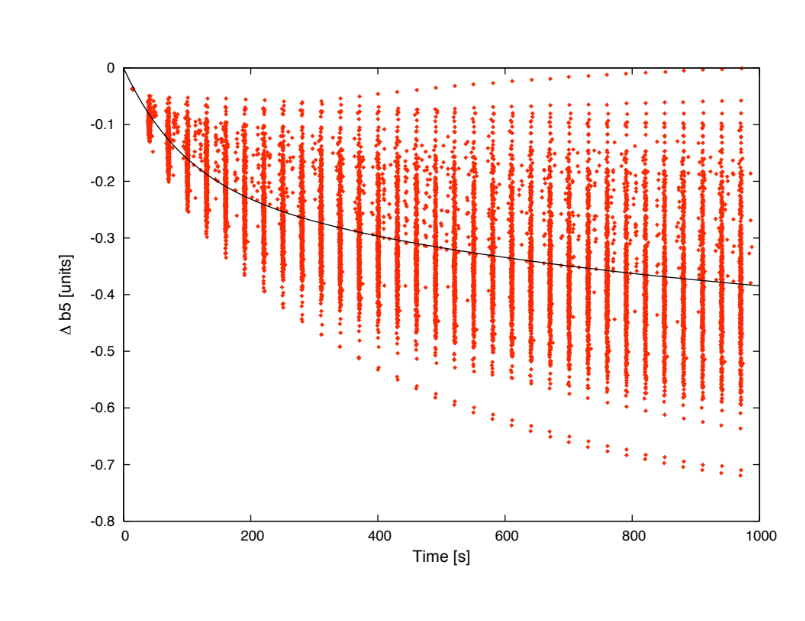
\includegraphics[width=0.7\textwidth]{./images/decay_b5_mb.pdf}
    \caption{Measured decay of the integrated decapolar field in LHC's main dipoles at injection
    energy. The fit is shown in black~\cite{deniau_magnetic_2009}.}
    \label{fig:decapoles:decay:decay_b5}
\end{figure}



% ==== Chromaticity
\paragraph{Chromaticity}
It has been shown in the previous sections, and particularly in
\cref{table:decapoles:bare_chromaticity:virgin_dq3} that measurements and simulations were off
regarding the third order chromaticity $Q'''$.
New simulations have hence been conducted to evaluate the effect of this decay on chromaticity.
\cref{table:decapoles:decay:simulation_chromaticity} compares simulations with and
without the decay of the $b_5$ component. The simulations use the 100 available error seeds to
calculate error bars.

\begin{table}[!htb]
    \centering
    \begin{tabular}{lll}
      \toprule
      Condition            & $Q'''_x [10^6]$ & $Q'''_y [10^6]$ \\
      \midrule
      No Decay             & $6.93 \pm 0.04$ & $-4.32 \pm 0.02$ \\
      $\Delta b_5 = -0.47$ & $4.05 \pm 0.04$ & $-2.54 \pm 0.02 $ \\
      \bottomrule
    \end{tabular}
    \caption{Comparison of $Q'''_x$ and $Q'''_y$ for Beam 1 with and without decay of the $b_5$
    component of the main dipoles at injection energy. Fields errors range from normal and skew
    sextupoles ($n=3$) to icosapole ($n=10$).}
    \label{table:decapoles:decay:simulation_chromaticity}
  \end{table}

Integrating the decay of the $b_5$ component of the main dipoles in the simulations shows a large
reduction of the third order chromaticity $Q'''$.
Using the values from the bare chromaticity measurement and updating
\cref{table:decapoles:bare_chromaticity:virgin_dq3} with the newly obtain data provides a more
accurate comparison of the model to the measurement, as shown in
\cref{table:decapoles:decay:virgin_dq3_recompare}.


\begin{table}[!htb]
    \centering
    \begin{tabular}{rrrr}
      \toprule
      Quantity     &  Measured $[10^6]$        &  Simulated $[10^{6}]$          &   \multicolumn{1}{c}{Ratio}     \\
      \midrule
        \multicolumn{1}{l}{Beam 1}    &                             &                                &             \\
                $Q'''_x$ &       $ 2.95 \pm 0.04$      & $ 4.05 \pm 0.04$               &  $0.73 \pm 0.01$  \\
                $Q'''_y$ &       $-1.82 \pm 0.04$      & $-2.54 \pm 0.02$               &  $0.72 \pm 0.02$  \\
      %\midrule
        \multicolumn{1}{l}{Beam 2}    &                             &                                &             \\
                $Q'''_x$ &       $ 3.06 \pm 0.07$      & $ 4.27 \pm 0.03$               &  $0.72 \pm 0.02$  \\
                $Q'''_y$ &       $-1.72 \pm 0.02$      & $-2.55 \pm 0.01$               &  $0.67 \pm 0.01$ \\
      \bottomrule
    \end{tabular}
    \caption{Measured and simulated third order chromaticity with octupole and decapole correctors
    turned off. The simulations include field errors from normal and skew sextupoles to icosapole
    ($n=3$ to $n=10$). The $b_5$ component of the main dipoles has been updated to include decay.}
    \label{table:decapoles:decay:virgin_dq3_recompare}
\end{table}




% ==== Chromatic Amplitude Detuning
\paragraph{Chromatic Amplitude Detuning}

Similar to chromaticity, new simulations have been conducted for chromatic amplitude detuning.
\cref{table:decapoles:decay:chromatic_ampdet} gives an overview of the newly computed values and 
the related ratios relative to the measurements, while \cref{figure:decapoles:decay:two_terms} gives
a visual clue.

\begin{table}[H]
  \centering
  \begin{tabular}{lrr}
  \toprule
   Type  & $\frac{\partial^2 Q_x}{\partial J_y \partial \delta}[10^{4}\mathrm{m}^{-1}]$ & $\frac{\partial^2 Q_y}{\partial J_y \partial \delta}[10^{4}\mathrm{m}^{-1}]$ \\
  \midrule
  $\delta = +0.001$ & & \\
  \hspace{2mm}Meas.  &   $-1.16 \pm 0.08$ &  $1.26 \pm 0.15$  \\
  \hspace{2mm}Sim.   &   $-2.35 \pm 0.01$ &  $1.50 \pm 0.01$  \\
  \hspace{2mm}Ratio  &   $ 0.49 \pm 0.03$ &  $0.84 \pm 0.10$  \\
  $\delta = -0.001$ & & \\
  \hspace{2mm}Meas.  &  $1.47 \pm 0.12$  &   $-1.18 \pm 0.13$ \\
  \hspace{2mm}Sim.   &  $2.46 \pm 0.01$  &   $-1.45 \pm 0.01$ \\
  \hspace{2mm}Ratio  &  $0.60 \pm 0.05$  &   $ 0.82 \pm 0.09$ \\
  \bottomrule
  \end{tabular}
  \caption{Comparison of the measured and simulated terms $\frac{\partial^2 Q_x}{\partial J_y
  \partial \delta}$ and $\frac{\partial^2 Q_y}{\partial J_y \partial \delta}$ via PTC, at two
  discrete momentum offsets. Simulations include errors from normal and skew sextupoles to 
  icosapole ($n=3$ to $n=10$), as well as the decay of the $b_5$ component of the main dipoles.}
  \label{table:decapoles:decay:chromatic_ampdet}
\end{table}

\todo{discrepancies between horizontal and vertical ?}

\begin{figure}[H]
  \centering
  \begin{subfigure}{0.8\textwidth}
      \centering
      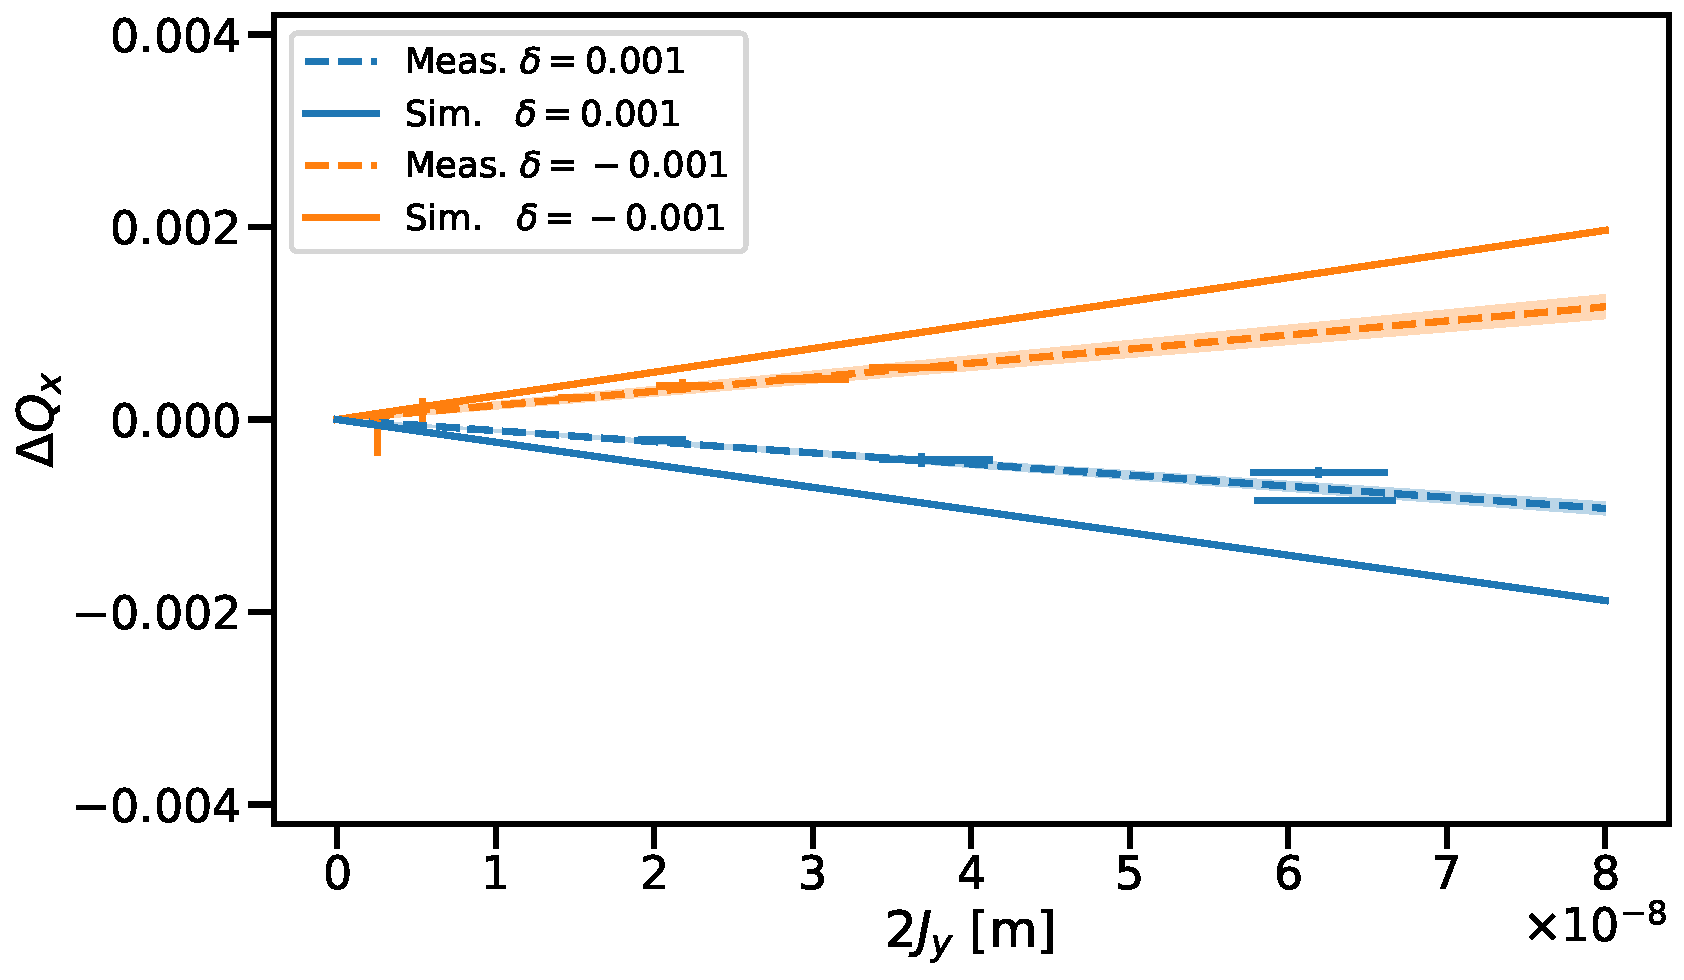
\includegraphics[width=\textwidth]{images/chromatic_amplitude_detuning/B2_Qxy_decay0.47.pdf}
      \caption{Horizontal tune shift depending on the vertical action: 
      $\frac{\partial^2 Q_x}{\partial J_y \partial \delta}$.}
      \label{figure:decapoles:decay:b2qxy}
  \end{subfigure}
  %
  \\[1em]
  %
  \begin{subfigure}{0.8\textwidth}
      \centering
      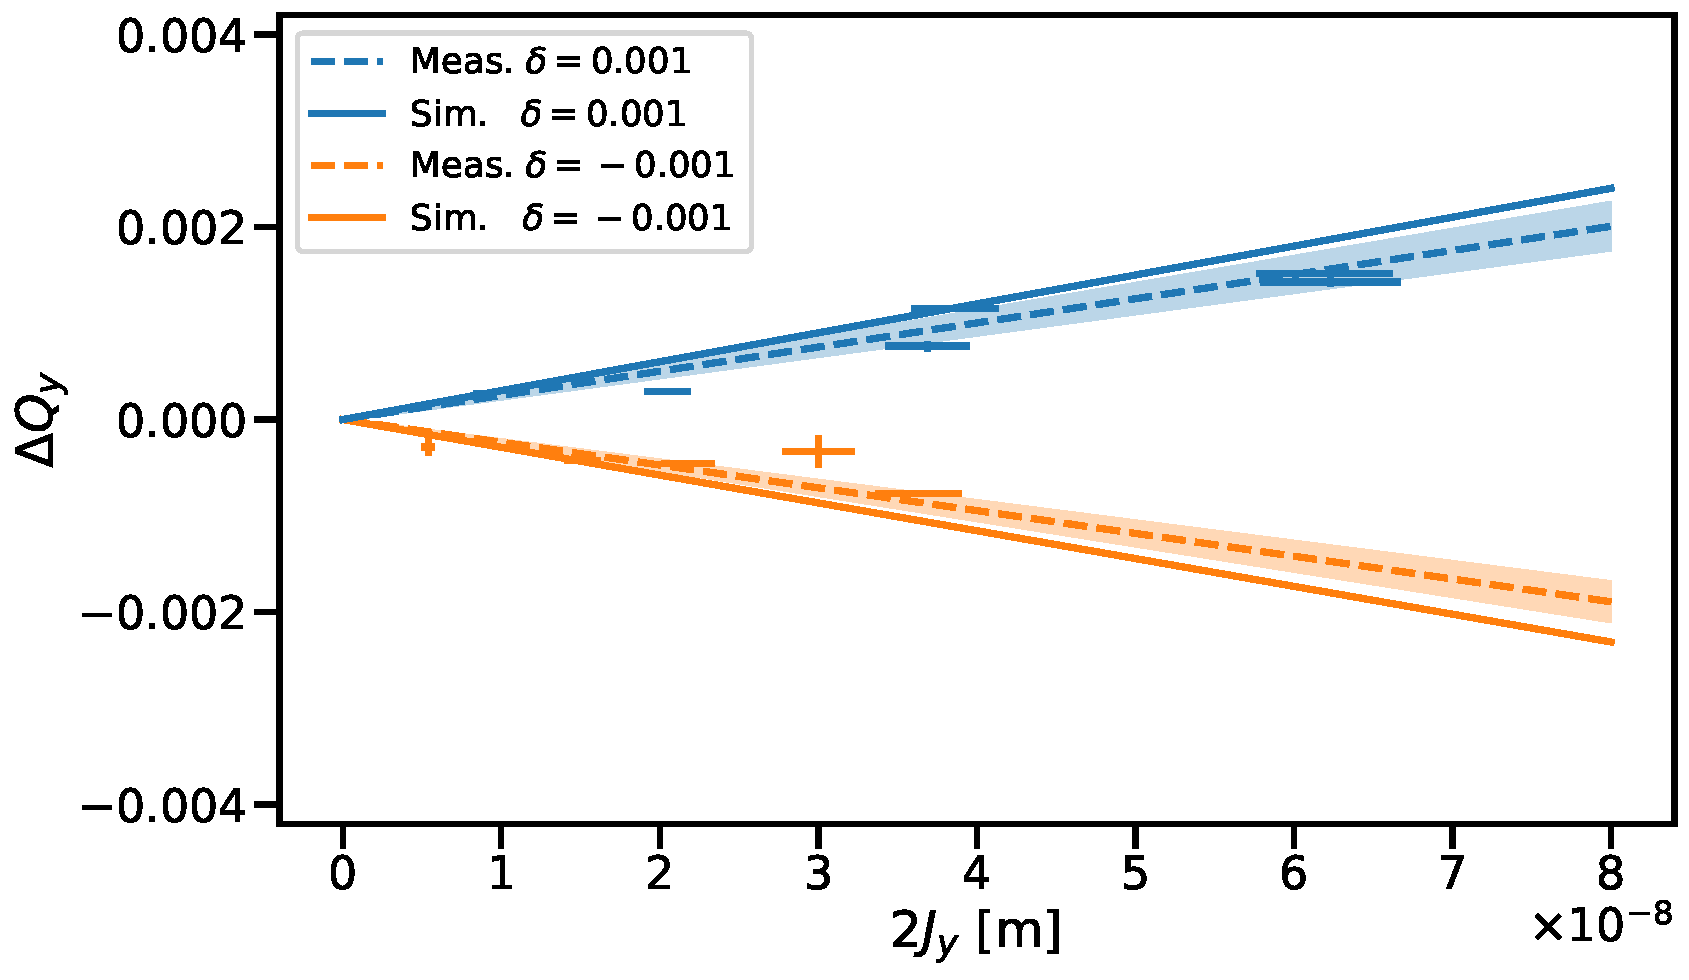
\includegraphics[width=\textwidth]{images/chromatic_amplitude_detuning/B2_Qyy_decay0.47.pdf}
      \caption{Vertical tune shift depending on the vertical action: 
      $\frac{\partial^2 Q_y}{\partial J_y \partial \delta}$.}
      \label{figure:decapoles:decay:b2qyy}
  \end{subfigure}
  \caption{Measured and simulated tune shift depending on the action at two different momentum
  offsets. Each fit corresponds to a chromatic amplitude detuning term evaluated at a certain
  $\delta$. Estimates from simulations are lowered due to the $b_5$ decay of the main dipoles.}
  \label{figure:decapoles:decay:two_terms}
\end{figure}

